\documentclass[a4paper,12pt,final]{article}

\usepackage{fullpage}
\usepackage{newpxtext,newpxmath}
\usepackage{amsmath}
\usepackage{graphicx}
\usepackage{parskip}

\newcommand{\HRule}{\rule{\linewidth}{0.5mm}}
\newcommand{\qrq}{\quad\rightarrow\quad}
\newcommand{\sen}{\textrm{sen}}
\newcommand{\tg}{\textrm{tg}}

\title{RMEC 13}
\author{Cesar M. Tessarin \and Daniel M. Doine}

\begin{document}

\begin{titlepage}
  \begin{center}

  \LARGE RMEC 13\\[1cm]

  \HRule\\[0.5cm]
  {\huge \bfseries Resolução dos Problemas Propostos}
  \HRule \\[8cm]

  Cesar M. Tessarin\\
  {\large \&}\\
  Daniel M. Doine

  \vfill

  {\large 1 de Setembro de 2010}

  \end{center}
\end{titlepage}

\section*{Problema 1}

\subsection*{Parte A}

Escrever na forma polar a equação cartesiana $y = x^2$.

\textbf{Resolução:}

Conhecendo `$x = r\cos\theta$' e `$y = r\,\sen\,\theta$':

$$
y = x^2
$$

$$
r\,\sen\,\theta = (r\cos\theta)^2 \qrq
r\,\sen\,\theta = r^2\cos^2\theta\quad(\div r)
$$

$$
\sen\,\theta = r\cdot\cos^2\theta\quad(\div \cos\theta)
$$

$$
r\cdot \cos\theta =
  \frac{\sen\,\theta}{\cos\theta} \qrq
r\cdot\cos\theta = \tg\,\theta
$$

$$
\boxed{r = \frac{\tg\,\theta}{\cos\theta}}
$$

\subsection*{Parte B}

Caracterizar a curva com a equação polar
$r = 2\cdot\cos\theta - 4\cdot\,\sen\,\theta$.

\textbf{Resolução:}

Multiplicando a equação por $r$, e sabendo que $r^2 = x^2 + y^2$:

$$
r^2 = r(2\cdot\cos\theta - 4\cdot\,\sen\,\theta)
  \qrq
r^2 = 2\cdot r\cos\theta - 4\cdot r\,\sen\,\theta
  \qrq
\underbrace{x^2 + y^2}_{r^2} = 2x - 4y
$$

Completando os quadrados perfeitos:
$$
x^2 - 2x + y^2 + 4y = 0
  \qrq
x^2 - 2x + 1 + y^2 + 4y + 4 = 1 + 4
$$

$$
\boxed{(x - 1)^2 + (y + 2)^2 = 5}\quad
\boxed{\textrm{Uma circunferência com o centro em }(1,-2)
\textrm{ e raio }\sqrt{5}}
$$

Fórmula geral de uma circunferência de centro $(a,b)$ e raio $r$:
$ \boxed{(x - a)^2 + (y - b)^2 = r^2} $

\newpage

\section*{Problema 2}

O primeiro passo a ser tomado é encontrar a coordenada de cada ponto. Sem
seguir a ordem alfabética, temos:

\subsection*{Ponto E}

Nota-se que está a mesma ``altura'' do ponto da parábola que cruza o eixo
\emph{y}. Logo, $y_E = 12$ \textit{(Função: $y = x^2 - 6x +
\textbf{\underline{12}}$)}.

Aplicando $y_E$ na função obtemos seu $x$:

$$ 12 = x^2 - 6x + 12 \qrq x^2 - 6x = 0 \qrq x(x - 6) = 0 $$

$$
\left\{\begin{array}{rl}
x'  \rightarrow 0 & (\textrm{Intersecção com eixo }y)\\
x'' \rightarrow 6 &
\end{array}\right.
$$

$$ \boxed{E(6,12)} $$

\subsection*{Ponto D}

Simplesmente observando o gráfico: \boxed{D(20,0)}

\subsection*{Ponto C}

Obviamente: \boxed{C(0,0)}

\subsection*{Ponto B}

A reta mostrada intercepta a parábola em dois pontos ($B$ e $E$). Sabemos
ainda que (-10,0) pertence a esta reta. Assim, podemos calcular sua função:

$$
m = \frac{\Delta y}{\Delta x} \qrq
m = \frac{12 - 0}{6 - (-10)} \qrq
m = \frac{12}{16} = \boxed{\frac{3}{4}}
$$

$$
(y - y_0) = m(x - x_0) \qrq
(y - 0) = \frac{3}{4}(x + 10) \qrq
\boxed{y = \frac{3}{4}x + \frac{15}{2}}
$$

$$
\frac{3}{4}x + \frac{15}{2} =
  x^2 - 6x + 12\quad(\times 4) \qrq
3x + 30 = 4x^2 - 24x + 48 \qrq
\boxed{4x^2 - 27x +18 = 0}
$$

$$
\Delta = b^2 - 4ac \qrq
\Delta = 27^2 - 4\cdot 4\cdot 18 \qrq
\Delta = 729 - 288 \qrq
\Delta = 441
$$

$$
x' = \frac{-b + \sqrt{\Delta}}{2a} \qrq
x' = \frac{27 + 21}{8} \qrq
\boxed{x' = 6}
$$

$$
x'' = \frac{-b + \sqrt{\Delta}}{2a} \qrq
x'' = \frac{27 - 21}{8} \qrq
\boxed{x'' = \frac{3}{4}}
$$

$x'$ já era um ponto conhecido. Assim, $x_B = x''$. Para calcular seu $y$:

$$
y_B = \frac{3}{4}x + \frac{15}{2} \qrq
y_B = \frac{3}{4}\cdot\frac{3}{4} + \frac{15}{2} \qrq
y_B = \frac{9}{16} + \frac{15}{2} \qrq
\boxed{y_B = \frac{129}{16}}
$$

$$ \boxed{B\left(\frac{3}{4},\frac{129}{16}\right)} $$

\subsection*{Ponto A}

Vértice da função. Pode ter seu $x$ descoberto facilmente pela média de
pontos simétricos, como E e o ponto de intersecção com o eixo $y$:

$$
\frac{6 + 0}{2} = 3\,,\quad\longrightarrow\quad
y_A = x_A^2 - 6x_A + 12 \qrq
y_A = 3^2 - 6\cdot 3 + 12 \qrq
y_A = 3
$$

$$ \boxed{A(3,3)} $$

\subsection*{Calculando a área}

Através da fórmula demonstrada por F.P. Garpelli, temos:

$$
S = \frac{1}{2}\times
\left\langle\begin{array}{ccccc}
  x_A & x_B & x_C & x_D & x_E\\
  y_A & y_B & y_C & y_D & y_E
\end{array}\right\rangle \qrq
%
S = \frac{1}{2}\times
\left\{\begin{array}{cccccc}
  x_A & x_B & x_C & x_D & x_E & x_A\\
  y_A & y_B & y_C & y_D & y_E & y_A
\end{array}\right\}
$$

$$
S = \frac{1}{2}\times
\left\{\begin{array}{cccccc}
3 & \frac{3}{4} & 0 & 20 & 6 & 3\\[.1cm]
3 & \frac{129}{16} & 0 & 0 & 12 & 3
\end{array}\right\}
$$

$$
S = \frac{1}{2}\times\left\{\left(3\cdot
\frac{129}{16} + 0 + 0 + 240 + 18\right) -
\left(3\cdot\frac{3}{4} + 0 + 0 + 0 + 36\right)\right\}
$$

$$
S = \frac{1}{2}\times\left\{\frac{387}{16} + 258 - \frac{9}{4} - 36\right\}
  \qrq
S = \frac{1}{2}\times\left\{222 + \frac{351}{16}\right\} \qrq
S = 111 + \frac{351}{32}
$$

Como $352 \div 32 = 11$, pode-se dizer que $\boxed{S \approx 122}$


\section*{Problema 3}

O primeiro passo, é posicionar a base e construir sobre ela um triângulo
com os dois lados não paralelos:

\begin{center}
  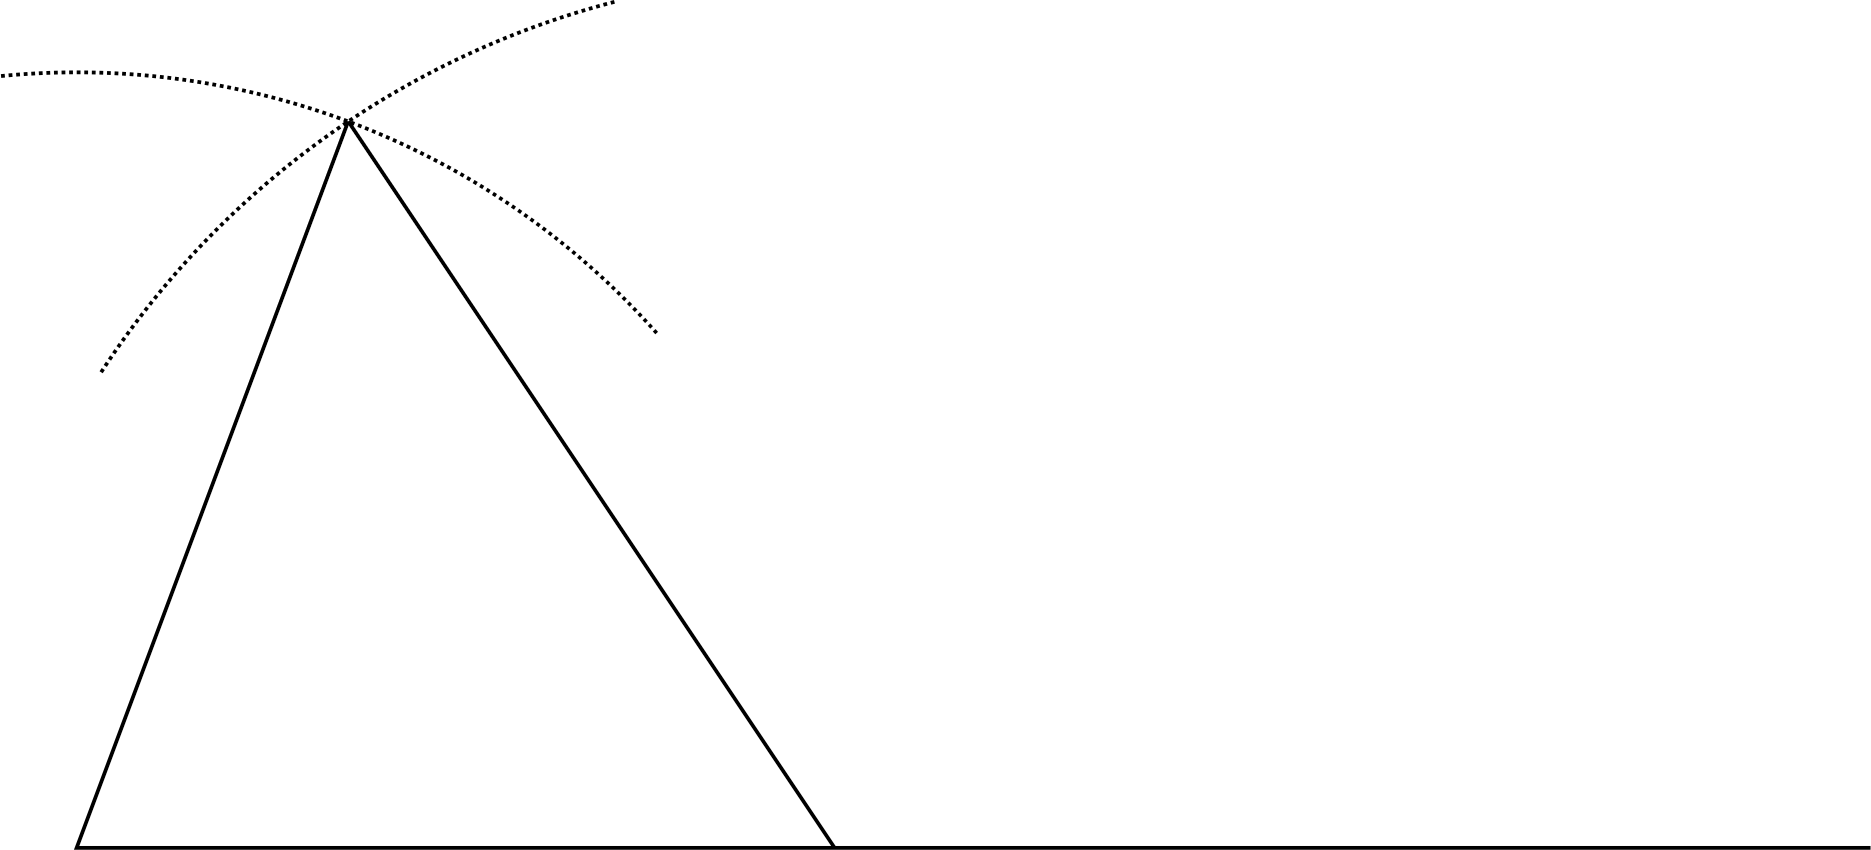
\includegraphics[scale=.12]{img/passo1}
\end{center}
\vfill

Em seguida, basta deslocar um dos lados para a outra extremidade da base e
adicionar o 4$^{\circ}$ lado (paralelo com a base):

\begin{center}
  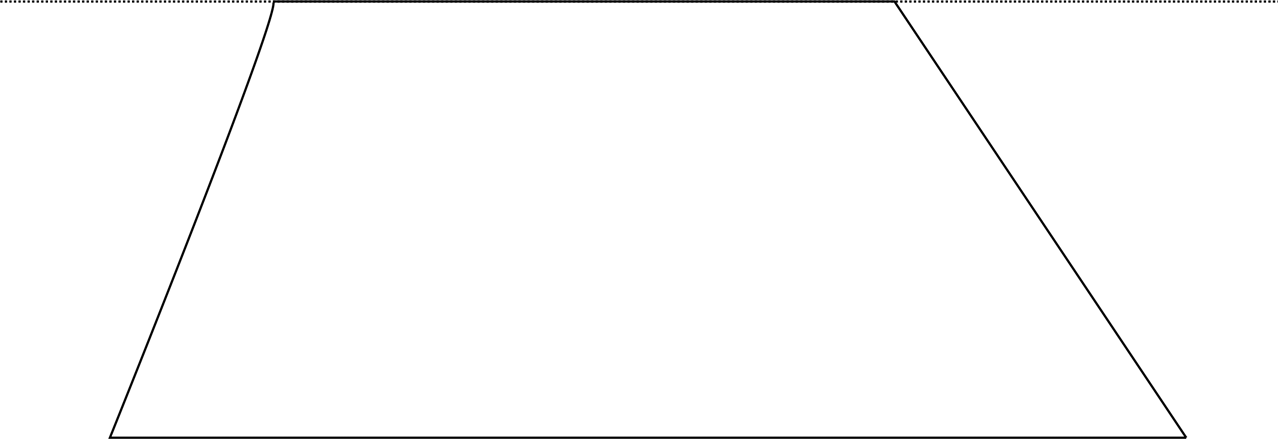
\includegraphics[scale=.18]{img/passo2}
\end{center}
\vfill

Formando o trapézio:

\begin{center}
  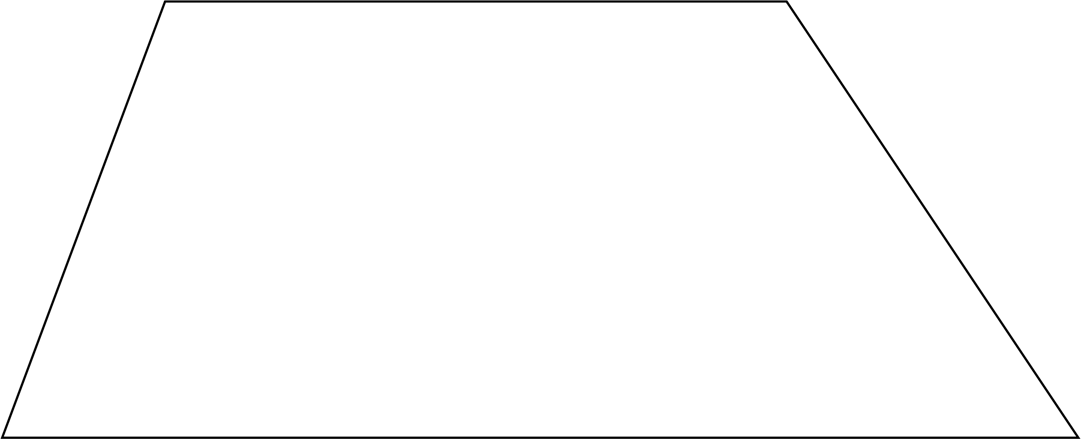
\includegraphics[scale=.25]{img/passo3}
\end{center}

\end{document}
